\scanpage{49}
% loc: cancelled continuation at head
\deleted{regarder $V$ seulement (où $\overline V=V\unsure{\otimes|\ominus}_{\mathbb Q}\overline{\mathbb Q}$)}
\[
\deleted{\overline V^{G}\subset\overline V\cap g(\overline V)}
\]
\deleted{et de prouver que c'est une identité [car $\overline V^G\cap V=V^G$].}

% loc: first equivalence
Or la relation $x\in\overset{\deleted{\unsure{-}}}{V}\cap g(\overline V)$ équivaut :
\begingroup\makeatletter\tagsleft@true\makeatother
\[
x\in\overset{\deleted{-}}{V},\quad g^{-1}x\in\overline V \tag*{ds}
\]
\endgroup
% loc: locus and second equivalence
et implique évidemment, si $\overline T$\inserted{$\subset\overline G$} est la \deleted{\unsure{déclinaison|clôture} de} \inserted{lieu de} $g$ sur $G_{\overline{\mathbb Q}}$
\[
x\in\overline V,\quad\deleted{\unsure{g^{-1}x}}\quad t\deleted{\unsure{^{-1}}}s^{-1}\in G_x(\mathbb C)\quad\text{pour }t,s\in\overline T(\mathbb C),
\]
et $=$ y équivaut.
% loc: stabilizer paragraph
En d'autres termes, si $G_x$ est le stabilisateur de \deleted{$G$}$x$, qui est un ss-gpe algébrique de $G$, \deleted{\unsure{on}} \inserted{la relation $x\in V\cap g(\overline W)$ équi-}vaut :
\[
\deleted{\unsure{g}}\overline R\in\overline{G_x}\deleted{\unsure{(\mathbb C)}},
\]
où $\overline R$ est l'adhérence de l'im. $\overline T\times\overline T\longrightarrow\overline G$, $(s,t)\longmapsto s^{-1}t$.

% loc: image subgroup and equality question
Or soit $\widehat R$ l'\unsure{image|im.ge} de $\overline R$ dans $G$, $H$ le sous-gr. qu'elle engendre, $H\subset G$. \deleted{Donc la propriété souhaitée équivaut à quelle \unsure{?}} La relation ds équivaut donc à $\deleted{R}H\subset G_x$ i.e. $H$ invarie $x$.
% loc: left insertion at opening of proposition
\inserted{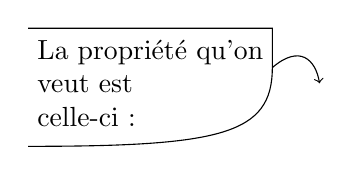
\begin{tikzpicture}[baseline=(n.base)]\node[align=left] (n) {La propriété qu'on\\veut est\\celle-ci :};\draw (-1.55,0.7) -- (1.55,0.7) -- (1.55,0.2) .. controls (1.55,-0.65) and (0.9,-0.8) .. (-1.55,-0.8);\draw[->] (1.55,0.2) .. controls (1.9,0.5) and (2.1,0.3) .. (2.15,0);\end{tikzpicture}}
% loc: heavily cancelled proposition and replacement
Pour tt $G$-module $V$, \deleted{et tt $x\in V$, tel que le stabilisateur $G_x$ contienne $R$, \inserted{i.e. tel que $R$ invarie $x$,} on a que $x\in V^G$ i.e. $G_x=G$.}
\deleted{Il suffit pour ceci que le \illegible{1} soit le ss-gpe engendré par $R$, soit égal à $G$. C'est aussi nécessaire} que les invariants de $H$ et de $G$ (pour tt repr. de $G$) soient les $=$s. Il suffit que l'on ait $H=G$, mais cette condition n'est pas nécessaire à priori, car un $k$-gpe de Borel de $G$ a cette propriété.
% loc: NB at left of cancelled lines
\margin{NB $\deleted{\unsure{\overline T}}\overline R,\overline H$ ne dépendent pas du choix de $g$ mod $G(\overline{\mathbb Q})$, \deleted{\unsure{à un près|a priori}}}
% loc: sloping note above 5
% slanted
\margin{\uline{Regarder} motifs \uline{associés} à \uline{courbes elliptiques}}
% loc: item 5, first half
5) Bien entendu, sans $=$ supposer que $k$ est alg. sur $\mathbb Q$, on peut regarder le foncteur (4.1). Mais il n'est plus en général pl. fidèle, $=$ si $k$ est de t.f. sur $\mathbb Q$, car pour $\unsure{\mathcal M|M}$ \inserted{$\otimes$-cat.} fixée de type fini $\subset\operatorname{Mot}(k)$, à condition d'agrandir $k$, on trouve que \inserted{les} $T_{\mathrm{DR}}(M)$ \uline{contiennent} $T_{\mathrm B}(M)$, donc les hom. des structures mixtes sont simplt les hom entre les $T_{\mathrm B}(M)$ : idiot !
% loc: closing lines of item 5
Pour $M$ fixé, on peut espérer tout au mieux avoir quelque résultat de disjonction de $T_{\mathrm B}$ et $T_{\mathrm{DR}}$ si $k$ est $\pm$ modérée (p.ex avoir des estimations de degré de transcendance minimum).
% No watermark lettering securely recoverable on this image; the reading supplied by C remains an audit question.
% archive sheet number: 48

